\subsection{APIS}
Dentro do projeto é utilizado as apis do Twitter e do Google Language, nessa parte será detalhado um pouco mais sobre as APIs e também como configura-las. Já foi abordado alguns aspectos técnicos na revisão, logo, esse detalhamento será voltado a parte de implementação.

A coleta será feita utilizando a API publica do twitter, o link para a documentação é \url{https://developer.twitter.com/en/docs}. Será trabalhado no projeto duas entidades: Tweet e Usuário. O tweet é a entidade que representa a publicação do usuário, enquanto o usuário contém informações necessárias sobre o seu perfil.

Para que seja possível acessar a API é necessário criar uma conta de desenvolvimento e gerar o \textit{token} de acesso\footnote{\url{https://apps.twitter.com/app/new}}. Com a chave em mãos é possível replicar o arquivo /dumont/sample\_env dentro do projeto Dumont para dumont/dev.env, e conforme demonstrado na Figura \ref{fig:twitteropts}, completar os campos necessários.

\begin{figure}
    \centering
    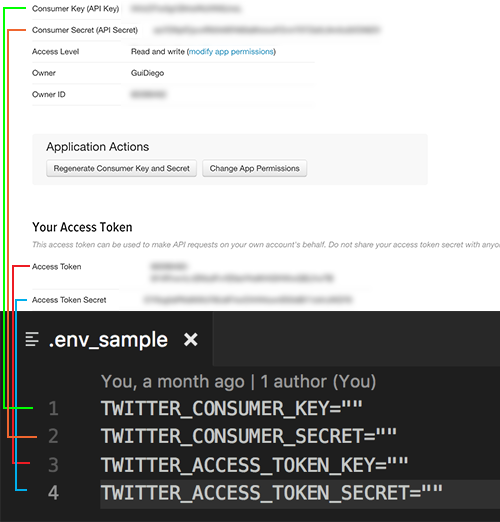
\includegraphics[width=.8\textwidth]{imagens/twitteropts.png}
    \caption{Imagem demonstrando onde cada chave deve ser inserida no código}
    \label{fig:twitteropts}
\end{figure}

Feito isso, é necessário conseguir o JSON de acesso do Google, esse arquivo serve como credencial para que seja possível obter os dados, Figura \ref{fig:twitteropts} pode-se observar que o valor \textit{GOOGLE\_APPLICATION\_CREDENTIALS} já esta definido como \textit{./google\_credentials.json}, ou seja, é necessário apenas baixar as credenciais, move-la para a pastas \textit{dumont/tasks} e renomear para \textit{google\_credentials.json}. Para conseguir acesso a essas credenciais acesse o site da api do Google Language\footnote{\url{https://cloud.google.com/natural-language/}} e clique em \textit{Try it Free}. Feito isso acontecera um redirecionamento para que seja escolhido uma conta google ou, em caso de nenhuma conta estiver previamente autenticada, a tela para efetuar a autenticação. Lembrando que é necessário para quem for replicar a pesquisa ter ao menos uma conta no google (pode ser o mesmo e-mail do gmail). Após selecionado será redirecionado para uma tela informando que o usuário tem 300 dólares gratuitos dentro da google cloud. O primeiro aceite é para receber notificações dos serviços da Google, e pode ficar marcado como "não". O segundo é o aceite dos termos de uso, e esse tem que estar marcado como "sim". Após isso basta clicar em "Agree and Continue". Basta completar algumas informações e informar um cartão de crédito valido (lembrando que isso é apenas um passo de segurança para a google). Feito isso você será direcionado para um \textit{dashboard} da google cloud, como mostrado na figura \ref{fig:googleflow}, basta clicar em \textit{Api \& Services > Credentials}, logo após acessar a tela de credenciais clique em \textit{Create credentials > Service Account Key} após mais um redirecionamento selecione o Serviço (caso não tenha um ainda, basta criar clicando em \textit{New service account}), mantenha a opção JSON marcada e clique em \textit{create}. Logo que fizer isso um JSON com um nome aleatório será baixado em sua máquina, basta mover e renomear como já dito previamente.

\begin{figure}
    \centering
    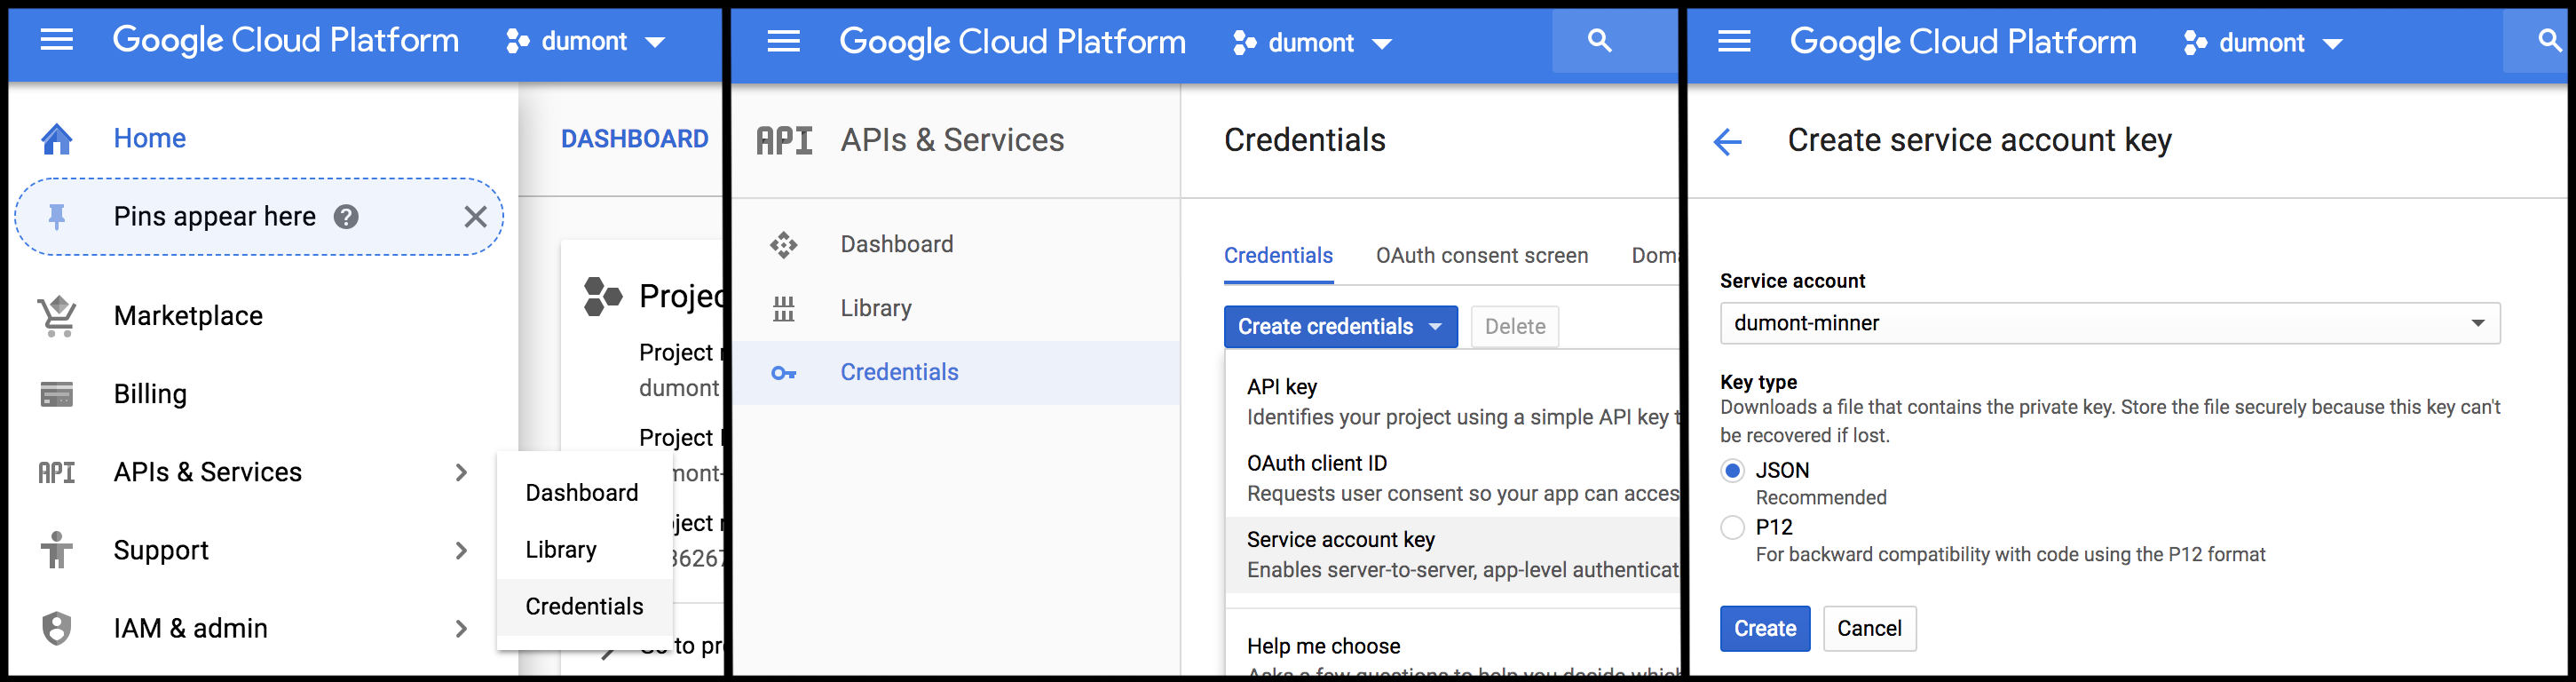
\includegraphics[width=1\textwidth]{imagens/googleflow.png}
    \caption{Imagem demonstrando passo a passo de como gerar o JSON de credencial}
    \label{fig:googleflow}
\end{figure}

Agora é possível executar os comandos, entretanto, existem configurações que devem ser retiradas e/ou alteradas para evitar problemas. Para isso vamos entrar na parte que envolve os processos de coleta e mineração de dados, com o intuito de entender as ultimas configurações e como todo o processo é executado.
